Изначально она должна различать искусственный интеллект, машинное обучение и глубокое обучение.

 % картинка /*искусственный интеллект, машинное обучение и глубокое обучение*/
 \begin{figure*}[h]
    \center{includegraphics{images/}}
    \caption{искусственный интеллект, машинное обучение и глубокое обучение}
 \end{figure*}

 Область изучения искусственного интеллекта является исследованием и дизайном интеллектуальных источников, 
 то есть системы, которая может принимать решения,
 основанные на характерной, считающийся умной.
 В искусственном интеллекте есть несколько методов, 
 которые моделирует эту характеристику и среди них является сфера машинного обучения,
 где решения сделаны (интеллект) на основе примеров,
 а не определяется программирования. 

 Алгоритмы машинного обучения требуют информации для удаления функций и элементов, 
 которые могут быть использованы для принятия будущих решений. 
 Глубокое обучение является подгруппой методов машинного обучения,
 которые обычно используют глубокие нейронные сети и нуждаются 
 в большом количестве информации для обучения. 

 По словам Сантаны есть некоторые различия между методами машинного обучения и методы глубокого обучения, 
 и основными из них являются необходимость и влияние объема данных, 
 вычислительной мощности и гибкости в моделировании проблем.

 Машинное обучение нуждается в данных для идентификации закономерностей, но есть два вопроса, 
 относящихся к размерности и стагнации производительности путем внедрения большего количества данных за пределы себя. 
 Подтверждено, что при этом происходит снижение значительной производительности. 
 По отношению к размерности то же самое происходит, 
 как есть много информации, чтобы обнаружить, 
 через классические методы измерения проблемы.

 % рисунок показывающий сравнение глубокого обучения с другими алгоритмами относительно объема данных.
 \begin{figure*}[h]
    \center{includegraphics{images/}}
    \caption{сравнение глубокого обучения с другими алгоритмами относительно объема данных.}
 \end{figure*}

 Область изучения искусственного интеллекта является исследованием и дизайном интеллектуальных источников, 
 то есть системы, которая может принимать решения, основанные на характерной, считающийся умной. 
 В искусственном интеллекте есть несколько методов, которые моделирует эту характеристику и среди них является сфера машинного обучения,
 где решения сделаны (интеллект) на основе примеров, а не определяется программирования.

 Алгоритмы машинного обучения требуют информации для удаления функций и элементов, 
 которые могут быть использованы для принятия будущих решений. 
 Глубокое обучение является подгруппой методов машинного обучения,
 которые обычно используют глубокие нейронные сети и нуждаются в большом количестве информации для обучения. 

 По словам Сантаны есть некоторые различия между методами машинного обучения и методы глубокого обучения, 
 и основными из них являются необходимость и влияние объема данных, 
 вычислительной мощности и гибкости в моделировании проблем.

 Машинное обучение нуждается в данных для идентификации закономерностей, но есть два вопроса, 
 относящихся к размерности и стагнации производительности путем внедрения большего количества данных за пределы себя. 
 Подтверждено, что при этом происходит снижение значительной производительности. 
 По отношению к размерности то же самое происходит, как есть много информации, 
 чтобы обнаружить,через классические методы измерения проблемы. 

 Классические методы также представляют точку насыщения по отношению к количеству данных,
 то есть максимальный предел для извлечения информации, которая не происходит с глубоким обучением,
 созданный для работы с большим объемом данных.

 По отношению к вычислительной мощности для глубокого обучения, 
 ее структуры являются сложными и требуют большого объема данных для ее подготовки, 
 которая демонстрирует свою зависимость от больших вычислительных мощности для реализации этих практик. 
 В то время как другие классические практики нужно много вычислительной мощности в качестве процессора, 
 глубокие методы обучения превосходят. 

 Поиск, связанный с параллельными вычислениями и использованием графических процессоров с CUDA-вычислительными
 унифицированными устройством архитектуры или унифицированными вычислениями устройства инициировали глубокое обучение, 
 как это было неосуществимо с использованием простого процессора. 

 В сравнении с обучением глубокой нейронной сети или глубоким обучением с использованием ЦП получается, 
 что добиться удовлетворительных результатов даже при длительном обучении было бы невозможно.

 Глубокое обучение, также известное как глубокое обучение, является частью машинного обучения,
 и оно применяет алгоритмы для обработки данных и воспроизведения обработки, 
 осуществляемой человеческим мозгом.

 Глубокое обучение использует слои математических нейронов для обработки данных, идентификации речи и распознавания объектов. 
 Данные передаются через каждый слой, при этом выход из предыдущего слоя предоставляет ввод следующему слою.
 Первый слой в сети называется входным слоем, а последний-выходной.
 Промежуточные слои называются скрытыми слоями, и каждый слой сети формируется простым и равномерным алгоритмом, 
 который включает в себя вид функции активации.

 % рисунок показывающий схемы простая нейронная сеть и глубокая нейронная сеть
 \begin{figure*}[h]
    \center{includegraphics{images/}}
    \caption{схемы простая нейронная сеть и глубокая нейронная сеть}
 \end{figure*}

 Самые крайние слои желтого цвета являются входными или выходными слоями, 
 а промежуточные или скрытые слои находятся в красном. 
 Глубокое обучение отвечает за последние достижения в области вычислительной техники, 
 распознавания речи, обработки языка и слуховой идентификации,
 основанные на определении искусственных нейронных сетей или вычислительных систем,
 которые воспроизводят путь человеческого мозга действует. 

 Еще одним аспектом глубокого обучения является извлечение ресурсов, 
 которое использует алгоритм для автоматического создания соответствующих параметров информации для обучения,
 обучения и понимания, задача инженера искусственного интеллекта.

 Глубокое обучение "--- это эволюция нейронных сетей.
 Интерес к глубокому обучению постепенно растет в средствах массовой
 информации и несколько исследований в области были распространены и
 его применение достигло автомобилей, в диагностике рака и аутизма,
 среди других приложений.

 Первые алгоритмы глубокого обучения с несколькими слоями нелинейных заданий представляют свои истоки в Алексее Григорьевиче Ивахненко, 
 который разработал метод групповой манипуляции данными и Валентин Григорьевич Лапа, 
 автор работы Кибернетика и методы прогнозирования в 1965 году.

 Оба использовали тонкие и глубокие модели с функциями полиномиальной активации, 
 которые исследовались с использованием статистических методов. 
 С помощью этих методов они отбирали в каждом слое лучшие ресурсы и передавались на следующий слой, 
 без использования обратного распространения, чтобы "обучить" полную сеть, 
 но использовали минимальные квадраты на каждом слое,
 где предыдущие были установлены от Самостоятельно в более поздних слоях, вручную.

 % строение первой глубокой сети, известной как Алексей Григоревич Ивахненко 
\begin{figure*}[h]
    \center{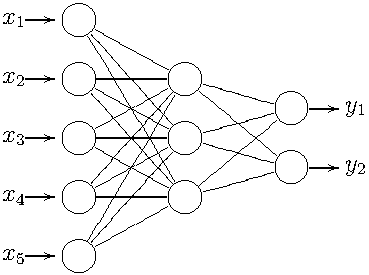
\includegraphics[]{images/NN-Persep.pdf}}
    \caption{строение первой глубокой сети, известной как Алексей Григоревич Ивахненко}
\end{figure*}

 В конце десятилетия 1970 зимы искусственного интеллекта произошло, 
 резкое сокращение финансирования исследований по этому вопросу.
 Воздействие ограничило прогресс в глубоких нейронных сетях и искусственном интеллекте. 

 Первые конволюционных нейронные сети были использованы Кунихико Фукусима, 
 с несколькими слоями группировки и извилин, в 1979. 
 Он создал искусственную нейронную сеть под названием Неокогнитрон 
 с иерархической и многослойной планировкой,
 которая позволила компьютеру идентифицировать визуальные паттерны. 
 Сети были аналогичны современным версиям, при этом «тренировка» была сосредоточена на стратегии усиления периодической активации в бесчисленных слоях. 
 Кроме того, конструкция Фукусима сделал возможным для наиболее релевантных ресурсов, 
 которые будут адаптированы вручную за счет повышения значимости некоторых соединений. 

 Многие руководящие принципы Неокогнитрон все еще используются,
 так как "сверху вниз" и новые методы обучения способствовали реализации различных нейронных сетей.
 Когда несколько шаблонов представлены в то же время, модель выборочного ухода может отделить их и идентифицировать отдельные шаблоны, 
 обращая внимание на каждый из них. Более современные Неокогнитрон можно определить шаблоны с отсутствием данных и завершить изображение, 
 вставив недостающее информацию, которая называется вывод. 

 Обратное распространение используется для глубокого обучения провал обучение прогрессировала от 1970 года, 
 когда Сепо Linnainmaa написал тезис, вставив код Фортрана для обратного распространения, без успеха до 1985.
 Румельхарт, Уильямс и Хинтон затем продемонстрировали обратное распространение в нейронной сети с представлениями распределения. 

 Это открытие позволило дебаты по AI достичь когнитивной психологии,
 которая инициировала вопросы о человеческом понимании и его связь с символической логики, 
 а также соединений. В 1989, Янн Летун выполнил практическую демонстрацию обратного распространения,
 с сочетанием конволюционных нейронных сетей для идентификации письменных цифр.

 В этот период вновь возникла нехватка средств на исследования в этой области, известная как вторая зима AI,
 которая произошла между 1985 и 1990, также затрагивающих исследования в нейронных сетях и глубокого обучения.
 Ожидания, представленные некоторыми исследователями, не достигли ожидаемого уровня, который глубоко раздражал инвесторов. 

 В 1995 году дана Кортес и Владимир Вадник создали поддержку векторной машины или поддерживающей векторной машины, 
 которая была системой картирования и идентификации подобной информации. 
 Длинная Краткосрочная память"=LSTM для периодических нейронных сетей была разработана в 1997 году, 
 Зепп Хохрайтер и Юрген Шмидхубер.

 Следующий шаг в эволюции глубокого обучения произошел в 1999,
 когда обработка данных и обработка графических процессоров (GPU) стали быстрее. 
 Использование графических процессоров и ее быстрая обработка представляли собой увеличение скорости работы компьютеров.
 Нейронные сети конкурировали с векторными машинами. Нейронная сеть была медленнее, 
 чем поддержка векторной машины, но они получили лучшие результаты и продолжали развиваться 
 по мере добавления дополнительной учебной информации. 

 В 2000 году была выявлена проблема под названием исчезающий градиент. 
 Задания, извлеченные в нижних слоях, не передавались в верхние слои однако,
 это произошло только в тех, с градиентом основе методов обучения. 
 Источник проблемы был в некоторых функциях активации, которые уменьшили его ввод,
 влияющим на диапазон выходных данных, генерируя большие области ввода,
 сопоставленные в очень малом диапазоне, вызывая падающий градиент. 
 Решения, реализы для решения проблемы, были слой за слоем перед 
 тренировкой и развитие долгосрочной и кратковременной памяти.

 В 2009 году фей-Фэй ли выпустила на свободу изображения
 с более чем 14 000 000 изображениями,
 сфокусирована на «обучении» нейронных сетей, указывая на то, 
 как большие данные повлияют на работу машинного обучения. 

 Скорость работы графических процессоров, вплоть до 2011 года, 
 продолжала увеличиваться, позволяя составу конволюционных нейронных 
 сетей без необходимости предварительного тренировки слоя за слоем. 
 Таким образом, стало печально, что глубинное обучение выгодно и
 с точки зрения эффективности и скорости. 

 В настоящее время обработка больших данных и прогрессирование искусственного интеллекта зависят от глубокого обучения, 
 которые могут разрабатывать интеллектуальные системы и способствовать созданию полностью автономного искусственного интеллекта, 
 который создаст влияние на все общество.